\chapter{Interpretazione astratta}
\section{Introduzione}
Nelle analisi precedenti l'approccio all'analisi statica è basato sull'informazione che
vogliamo osservare dell'esecuzione del programma, in particolare per proprietà relativamente semplici,
molto vicine alla sintassi che non descrivono informazioni sul contenuto delle variabili,
quindi in relazione agli elementi del programma piuttosto che al contenuto di tali elementi.

Per questo tipo di analisi, o in modo algoritmico fornendo direttamente l'equazione da risolvere, o 
in modo semantico, fornendo una semantica di elaborazione dell'informazione, costruita 
in modo induttivo sulla sintassi del linguaggio, riusciamo a fornire una soluzione sull'informazione
ricercata.

Il problema si pone quando vogliamo guardare ciò che accade al programma durante l'esecuzione, 
siamo quindi interessati a guardare all'interno delle stato della macchina, e non più alla relazione 
tra gli elementi del programma. Questo diventa relativamente un problema, poiché fornendo una 
semantica, tale semantica non risulterebbe distributiva, di conseguenza ci sarà necessariamente 
una perdita di informazione legata al fatto che risolvendo l'analisi localmente su punti di programma 
del \texttt{CFG} perdiamo informazione rispetto alla semantica desiderata, ovvero quella che considera 
tutti i cammini di esecuzione, ovvero la \textbf{MOP}. Si tratta del prezzo da pagare per rendere 
decidibile un calcolo su un informazione che si avvicina sempre di più all'informazione concreta, ovvero 
l'evoluzione dello stato della macchina.

Guardare all'interno dello stato della macchina significa avvicinarsi sempre di più 
all'informazione concreta, ma richiede un prezzo che è quello di staccarci 
dalla soluzione \textbf{MOP}, ottenendo attraverso la soluzione del calcolo 
di un sistema di disequazioni, una soluzione approssimata.

Nel momento in cui siamo interessati a guardare all'interno dello stato della macchina,
allora abbiamo bisogno, per mantenere delle garanzie sul calcolo della semantica astratta, 
di un'infrastruttura chiamata \textbf{interpretazione astratta}.

\begin{tcolorbox}[title=Interpretazione astratta]
    L'interpretazione astratta è un framework formale che permette di descrivere 
    dettagliatamente la relazione tra il momento concreto, di cui vogliamo dire 
    qualcosa, e il momento astratto, su cui possiamo dire qualcosa, garantendo informazioni 
    certe, anche se approssimate, su alcuni aspetti di interesse
    del mondo concreto.
\end{tcolorbox}
L'obiettivo è di verificare in modo automatico proprietà di interesse dei programmi e 
l'astrazione è il procedimento utilizzato per arginare il problema della non decidibilità
della semantica concreta.

\section{L'idea di base dell'interpretazione astratta}
L'idea di base è che un qualunque oggetto concreto sia formato da due elementi, un origine e 
un insieme finito di punti.

Supponiamo di definire nel nostro dominio concreto un oggetto fiore e vediamo come è possibile 
ottenerlo attraverso l'applicazione di operazioni concrete e partendo da operazioni concrete.
\begin{figure}[H]
    \centering 
    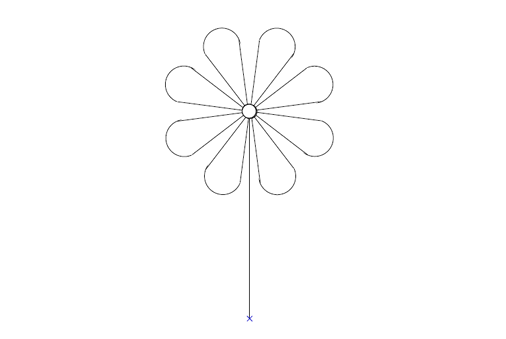
\includegraphics[scale=0.5]{img/flower.png}
\end{figure}
Tali oggetti non sono altro che dei numeri interni, quindi immaginiamo il fiore come una sequenza 
di operazioni che applichiamo ad elementi più piccoli, ovvero elementi del dominio stesso.
\subsection{Operazioni concrete}
Le operazioni che possiamo applicare sono le seguenti:
\begin{itemize}
    \item Costante: operazione che fornisce un petalo.
    \item Rotazione: $r[a](o)$ è un'operazione che ruota di $a$ gradi l'oggetto $o$.
    \begin{figure}[H]
        \centering 
        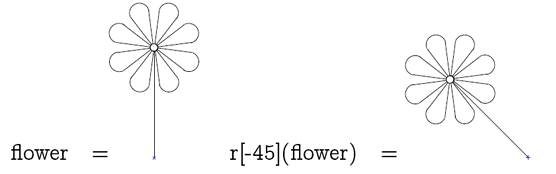
\includegraphics[scale=0.5]{img/rotation.png}
    \end{figure}
    \item Unione: $o_1 \cup o_2$ è un'operazione che unisce due oggetti $o_1$ e $o_2$, sovrapponendo 
    le origini.
    \begin{figure}[H]
        \centering 
        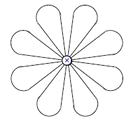
\includegraphics[scale=0.5]{img/corolla.png}
        \caption{$\texttt{corolla} = \texttt{petal} \cup r[45]\texttt{petal} 
        \cup r[90]\texttt{petal} \cup r[135]\texttt{petal}
        \cup r[180]\texttt{petal} \cup r[225]\texttt{petal} 
        \cup r[270]\texttt{petal} \cup r[315]\texttt{petal}$}
    \end{figure}
    \item \textit{stem}(o): è un'operazione che aggiunge un gambo all'oggetto $o$, il gambo viene sovrapposto 
    all'origine e la nuova origine è quella del gambo.
    \begin{figure}[H]
        \centering 
        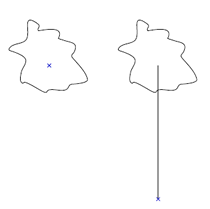
\includegraphics[scale=0.5]{img/stem.png}
    \end{figure}
\end{itemize}
Per la costruzione della corolla possiamo trovare un operatore monotono che applicato iterativamente 
fino al raggiungimento di un punto fisso, ci permette di ottenere la corolla. Possiamo costruire oggetti 
concreti per punto fisso a partire da oggetti più semplici, che è ciò che avviene con la semantica.
\[
  \texttt{corolla} = lfp^{\subseteq} F  
\]
\[
    F(X) = \texttt{petal} \cup r[45](X)
\]
\begin{figure}[H]
    \centering
    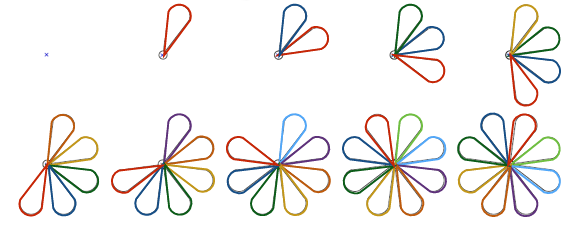
\includegraphics[scale=0.5]{img/fixpointcorolla.png}
\end{figure}
Abbiamo quindi introdotto un dominio concreto di oggetti su cui abbiamo definito delle operazioni.
\subsection{Approssimazione verso l'alto}
Operare su tali oggetti può comportare situazioni di non decidibilità, l'idea è quindi di approssimare 
tali oggetti concreti.
Definiamo la relazione di approssimazione, ovvero cosa vuol dire essere meno precisi. Nel caso degli 
oggetti, quello che è essere meno precisi è avere la stessa origine, ma che contengono più pixel, ovvero 
aggiungere rumore rispetto all'informazione originale.
\begin{figure}[H]
    \centering
    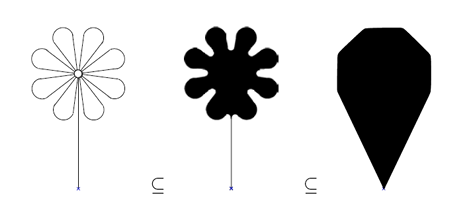
\includegraphics[scale=0.5]{img/upperapprox.png}
\end{figure}
In questo particolare caso abbiamo perso parte del dettaglio della figura, in particolare la corolla.
Aver più pixel aggiunge quindi rumore.

\subsection{Oggetti astratti}
L'oggetto astratto è una rappresentazione di un oggetto concreto che vogliamo fornire in 
forma approssimata. Decidiamo di rappresentare l'insieme di pixel dal suo contorno.
Questo è l'ordine che inseriamo nel dominio di computazione, propagando l'ordinamento,
che nel dominio concreto è dato dal contenimento, sul dominio astratto.
Un oggetto è quindi più astratto se è la rappresentazione di un oggetto concreto più grande.

\begin{figure}[H]
    \centering
    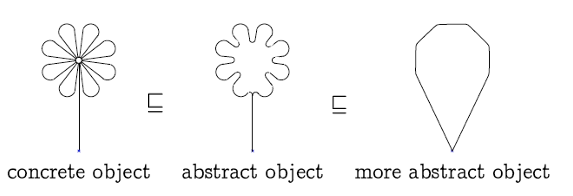
\includegraphics[scale=0.6]{img/abstractobj.png}
\end{figure}
